\chapter{Defect detection and prevention techniques} \label{chap:otherdets}

This paper argues for the relevance of code reviews and software inspection in today's software
industry setting.
To do so, we must ``set the scene" and discuss the current state-of-the-art in defect strategies in
software engineering.
It is thus worthwhile to introduce and survey other defect detection techniques.
We can analyse their relative strengths and weaknesses, and discuss why subtle
errors might escape these techniques.\\
\\
This will not be an in-depth survey of each technique --- we are focusing on code reviews, rather
than these techniques.
Instead, we will speak to each of these with a summary of recent achievements and usage, a
description of what the technique is at a high level, and what the author believes about the
technique and its usage.\\
\\
To address our claims that code reviews have long term benefits, such as defect
prevention properties, we ought to look at different defect prevention
techniques as well.
We will examine three areas of defect detection, and three areas of defect
prevention.
The two defect detection areas are
\begin{itemize}
	\item Test-driven development (Section \ref{sec:otherdets:TDD})
	\item Automated static analysis (Section \ref{sec:otherdets:static})
\end{itemize}
The two defect prevention techniques are
\begin{itemize}
	\item Defensive programming (Section \ref{sec:otherdets:defProg})
	\item Formal methods and model checking (Section \ref{sec:otherdets:modelCheck})
\end{itemize}

\section{Test-driven development} \label{sec:otherdets:TDD}

Continuous development, and the continually refactoring and refining a program according to client
expectations are the basis of Agile programming \cite{sommerville1989software}.
One of the branches of Agile programming is Extreme Programming (XP), defined by Beck
\cite{beck2006extreme} from which the ideas of test-driven development evolved.\\
\\
Test-driven development states that tests should be written before the program is run, as a means of
specifying a running ``contract" of how the program should work.
Some of its variants include the {\em red-green-refactor} methodology and acceptance-test-driven
development.\\
\\
{\em Red-green-refactor} (or RGR), introduced by Shore \cite{shore2005RGR}, is a formalisation of the test-driven mantra in
terms of an easy to visualise process.
A developer codes a purposely wrong and small software module, then codes a test that catches the
error (and thus the test is {\em red}).
Once the test catches the error, and thus proves it is working, the developer makes a small change
to the wrong module to correct it, then re-runs the test.
The test should now be passing ({\em green}), and the developer can then {\em refactor} the code to
improve it.
The process repeats itself and slowly makes incremental changes to the system.
This is demonstrated in Figure \ref{figure:RGR}.\\
\\
\begin{figure}
\centering
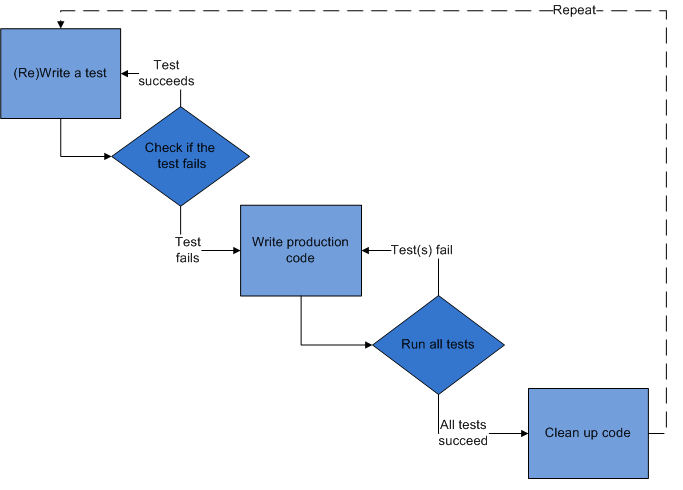
\includegraphics{media/Test-driven_development}
\caption{This is the red-green-refactor model, as taken from \cite{RGR:image}, though not entirely
truly transcribed.
However, the basic ideas of RGR can be seen within this model.}
\label{figure:RGR}
\end{figure}
\\
However, this practice is only as effective as the tester.
If the test suite itself is fragile, it is clear that the tests are almost useless, and could lure a
development team into a false sense of security.
Furthermore, RGR only works a unit-test level, without looking beyond small code modules and at the
system as a whole.
In my opinion, this is where system testing and acceptance tests are necessary.\\
\\
Acceptance-test-driven development, as defined by Quartel \cite{AcceptQuartel} and Hendrikson
\cite{AcceptHendr} (though they do not appear to be
the originators of the practice) involves a team-based and client-based approach to test-driven
development.
Instead of writing tests for code, the team aims to construct acceptance tests with the client
early, and continually update these tests.\\
\\
I personally do not like this methodology --- acceptance tests are not at all flexible. 
I think it carries the risk of aiming toward a goal (customer vision/expectations) without constant
feedback on whether the goal is appropriate (because it takes so long to satisfy an acceptance test).
This might be because the terminology ``acceptance test" is an artefact of older life-cycle
approaches, and does not translate well to an Agile practice.
One might argue that ``Acceptance Test-Driven Development" is essentially Agile, but this does not
take into account the ideas of ``regression acceptance test suites" (which seem counter-intuitive",
or the expense required to change an acceptance test.\\
\\
Overall, these two methodologies are some differing ideas about test-driven development.
I believe they are essential parts of the software engineering process.
To develop good software, one ought to have code tested continuously, and the tests give the
original developer some measure of confidence in their code.\\
\\
However, it is clear that tests rely upon the confidence of the tester, and the unit tests are only
as good as the person who wrote the software being tested.
Furthermore, the unit tests are an encoding of that developer's understanding of the module's
functionality, and it captures their assumptions and conceptions about the software.
This understanding can easily be flawed or misguided, and that in turn affects the software quality
and the test suite quality until a larger problem (an error or failure) occurs.
Thus, test-driven development (to my mind) cannot find the larger or subtler problems at a code module level, or is not flexible enough to adapt to
finding these large problems.

\section{Automated static analysis} \label{sec:otherdets:static}

Imagine having a spell- and grammar-checker in your document editor, except it analysed your code,
instead.
It detected bad code patterns (code smells, see Atwood for a more comprehensive list
\cite{AtwoodCodeSmells}), potential memory leaks and made optimisations
for you (and it also does spell- and grammar-checking on your documentation).
This is the domain of automated static analysis --- having a machine inspect code and detect the
presence of possible faults \cite{chess2007secure}.\\
\\
Much work has been done to improve the quality of static analysis since Fagan's time.
Biffl \cite{Biffl2012BenefitAutomatedStaticAnalysis} found that small to medium scale enterprises
found benefits in introducing static analysis tools.
There was a unified response from both management and development teams that the static analysis
tools were useful and helpful.
Furthermore, the authors found that it typically took under one hour to
introduce these analysis tools.\\
\\
Interestingly, the authors were able to introduce ``architectural conformance" of a system into
these enterprises.
They could determine circular dependencies or points where the architecture and abstraction layers
were circumvented for ease of code production.
This shows some of the power of static code analysis, in that it has begun to, at a high level,
detect problems in an entire system.\\
\\
Contrastingly, Thung et. al \cite{Thung:2012:EWD:2351676.2351685} find that static analysis still
missed many defects.
They compared the number of false negatives that the static analysis systems had found,
and noted that although they found many defects there were a large range of defects that common
static analysis tools missed.
Their findings suggested that defect detection through static analysis still had a ways to go, with
regards to missing a significant number of defects.\\
\\
Automated static analysis is thus a contender to replace humans in code reviews, since automated
static analysis is essentially doing what a human code reviewer does.
They detect faults in the code by examining it against a set of pre-determined criteria.
These faults can be corrected early before they escalate into major errors and failures.
My own opinion is that such analyses are still rudimentary, and that we should not so quickly
discard the critical thinking of a human.\\
\\
Furthermore, Biffl et. al \cite{Biffl2012BenefitAutomatedStaticAnalysis} suggest that there is a need to
select a ``template" for system-wide static analysis.
In my opinion, this further suggests that static analysis is not amenable to large changes in
system-wide software architecture, and could potentially take longer to adapt than a human would
This is simply conjecture and opinion, though, but to my mind it justifies the need for human code
reviewers, rather than just automated static analysis tools.

\section{Defensive programming} \label{sec:otherdets:defProg}

Defensive programming, also known as ``secure programming", looks at eliminating assumptions from
a developer's mindset.
The code developed under defensive programming is centred around accounting for all possibilities,
employing assertions, whitelisting over blacklisting (checking for a correct state and running code,
rather than checking for an incorrect state and throwing an error) and avoiding double negations (e.g. checking that
the result is not incorrect is a double negation).
The entire basis for defensive programming is to prevent defects.
Part of its motivation is to address security concerns and thus decrease the vulnerability of
software components.\\
\\
Campbell \cite{campbell1998defensive}, as well as Qie et. al \cite{qie2002defensive}, have looked at
how defensive programming is useful in preventing defects in embedded systems (where testing may
be more difficult or expensive), as well as building security into programs to make them DoS
(denial-of-service) resistant.
However, Roop \cite{roop2009defensive} argues against defensive programming when employed in an extreme fashion
mainly due to the difficulty in maintaining and readability of the resultant code.\\
\\
I agree with Roop --- I recently constructed a networking protocol for file transfers in an
assignment, and found that it was very difficult to reason about the code I had written.
In some regards, we employed some of the methodologies and ideas behind defensive programming ---
making no assumptions, having a state-based protocol and accounting for all states, and whitelisting
the correct state, rather than blacklisting incorrect states.
However, this lead to hard to read code that I found difficult to debug.
Tracing which part of the protocol was being executed was hard to determine, and although it worked,
much refactoring could have been performed to ensure that it was more readable.\\
\\
Furthermore, defensive programming, though a good set of guidelines to improve the readability and
maintainability of code, places all the onus upon the developer.
Some of the guidelines, such as ``whitelisting over blacklisting", or ``avoiding double negations",
seem easily representable in a static code analysis tool.
However, others, such as ``checking for all possible errors", can only be enforced by the developer
themselves.
Again, as with test-driven development, much responsibility is placed upon the developer to adhere
to these guidelines.
But a developer is a human and is error-prone --- who can enforce the guidelines of defensive
programming, if we cannot trust the developer themselves to do so?

\section{Formal methods and model checking} \label{sec:otherdets:modelCheck}

\begin{quote}
Program testing can be used to show the presence of bugs, but never to show their absence.
\end{quote}

So claimed Dijkstra \cite{dijkstra1970notes}, on the subject of verifying the correctness of a program.
At the time, many scientists argued for proofs of correctness for programs --- Dijkstra claimed that
this would be an expensive and unfeasible task.
Indeed, as software has grown and expanded, proving that components work has become an arduous and
logistically complex task.\\
\\
Instead of having people and developers prove the correctness of their code, we instead turn to
machines to do so.
{\em Formal methods} are a way to prove the correctness of code, by a formal, verifiable
specification that can be run against the resultant system.
In doing so, we can employ model checkers to verify whether a system will do exactly as it was
specified, by using an automated prover to show that it does.\\
\\
We briefly discuss Klein et. al's contribution to the area of formal methods and model checking, by way of
discussing, without detail, his provably correct kernel \cite{klein2009sel4}.
Klein et. al proved that their implementation of an SELinux microkernel, seL4, was correct and
matched its specification, by means of an automated proving specification in Haskell.
It showcased the power of formal methods, when employed by familiar and expert users who had
mastered the concepts of formal methods, and is now being employed in embedded devices the world
over.\\
\\
Formal methods are clearly desirable for safety critical programs.
Being able to formally show that a program will do exactly what is expected of it is a desirable and
useful property.
However, it is timely to learn and set up such a programme --- model checking and formal methods are
not commonly used, and are an expert field unto themselves.
Furthermore, how can we show that the specification itself is correct?
That there are no defects within the model checker?\\
\\
High setup costs make it hard to motivate the usage of formal methods for the mainstream software
industry, beyond safety critical software.
I hope to, in this paper, speak to more than just those who need to write safety-critical software,
and instead discuss software engineering at large.

\section{Open questions}

We have examined two defect detection, and two defect prevention techniques, and in each we have
identified some areas where they have shortcomings:
\begin{itemize}
	\item many of them rely on the sole developer to be responsible for defect detection or prevention
	\item they might have high initiation costs and be difficult to set up
	\item it is difficult to see subtleties or verify/prevent the existence of subtle design errors
		using these methods
\end{itemize}

The issues we have highlighted with these defect detection/prevention techniques are ones that I hope
to show code reviews can mitigate in this next chapter.
